% TEMPLATE AUTHOR: https://bitbucket.org/m_by/fiit-stu-thesis-template-for-latex
% EDIT: Jozef Gáborík


% SETTINGS - LATEX
% to change name, title, supervisor etc. go to preamble/preamble.tex
\newcommand{\myFontSize}[0] {12pt}
\newcommand{\mySpacing}[0] {1.5}
\newcommand{\myBibliography}[0] {bib/refs, appendices/refs1}

\documentclass[\myFontSize,a4paper,twoside,openright,english]{book}
\usepackage{glossaries}
\usepackage{float}
\usepackage{longtable}
\setacronymstyle{long-short}
\newacronym{ml}{ML}{Machine learning}
\newacronym{dl}{DL}{Deep learning}
\newacronym{dp}{DP}{Differential privacy}
\newacronym{dnn}{DNN}{Deep neural network}
\newacronym{cnn}{CNN}{Convolutional neural network}
\newacronym{rnn}{RNN}{Recurrent neural network}
\newacronym{its}{ITS}{Intelligent transport system}


\usepackage[utf8]{inputenc}
\usepackage[T1]{fontenc}
\usepackage[english]{babel}
\usepackage[a4paper]{geometry}
\usepackage[
    left = \glqq,% 
    right = \grqq,% 
    leftsub = \glq,% 
    rightsub = \grq%
]{dirtytalk}

% SETTINGS - NAMES
\newcommand{\myTitle}[0] {Tuning ML hyperparameters with privacy preservation}
\newcommand{\myName}[0] {Hlib Kokin}
\newcommand{\mySupervisor}[0] {Ing. Oleksandr Lytvyn}
\newcommand{\myEvidenceNumber}[0] {FIIT-XXXX-XXXXX}
\newcommand{\myDate}[0] {January 2023}
\newcommand{\myStudyProgram}[0] {Informatics}
\newcommand{\myDegreeCourse}[0] {Informatics}
\newcommand{\myInstitute}[0] {Institute of Informatics and Software Engineering, FIIT STU, Bratislava}

\usepackage[parfill]{parskip}
\usepackage{enumitem}

\usepackage{graphicx}
\usepackage{float}
\usepackage{longtable}
\usepackage{setspace}

% Spacing
\setstretch{\mySpacing}

\setcounter{secnumdepth}{3}
\setcounter{tocdepth}{3}

\usepackage{tabularx}
\newsavebox\mybox
\usepackage{fancyhdr}
\pagestyle{fancy}
\lhead{\nouppercase{\leftmark}}
\chead{}
\rhead{}
\lfoot{}
\cfoot{\thepage}
\rfoot{}


%style=iso-numeric
%style=authortitle-dw
\usepackage[backend=bibtex,defernums=true]{biblatex}
\defbibheading{references}[Literature]{ 
  \chapter*{#1}
  \markboth{#1}{#1}
}
\defbibheading{referencessec}[Literature]{ 
  \section*{#1}
  \markboth{#1}{#1}
}
\bibliography{\myBibliography}


% Listing as figure
%\usepackage{libs/minted}
%\usepackage[section]{minted}

\usepackage{listing}

% openright does not work :(
\let\tmp\oddsidemargin
\let\oddsidemargin\evensidemargin
\let\evensidemargin\tmp
\reversemarginpar

\usepackage{lscape}
\usepackage{afterpage}

\usepackage{lipsum}
\usepackage{todonotes}


\begin{document}

% Minted
% pygmentize -L styles
%\usemintedstyle{autumn}


% Title page

\begin{center}
\thispagestyle{empty}
{\Large Slovenská technická univerzita v Bratislave}
\par\end{center}{\Large \par}

\begin{center}
{\Large Fakulta informatiky a informačných technológií}
\par\end{center}{\Large \par}

\smallskip{}

\begin{center}
\myEvidenceNumber
\par\end{center}
\vfill{}

\begin{center}
\textbf{\Large \myName}
\par\end{center}{\Large \par}

\medskip{}


\begin{center}
\textbf{\LARGE \myTitle }
\par\end{center}{\huge \par}

\medskip{}


\begin{center}

{\Large Bakalárska práca}
\par\end{center}{\Large \par}

\vfill{}

Vedúci práce: \mySupervisor

\medskip{}
\myDate

\pagenumbering{roman}

\newpage
\thispagestyle{empty}
\mbox{}
\newpage



\begin{center}
\thispagestyle{empty}
{\Large Slovenská technická univerzita v Bratislave}
\par\end{center}{\Large \par}

\begin{center}
{\Large Fakulta informatiky a informačných technológií}
\par\end{center}{\Large \par}

\smallskip{}

\begin{center}
\myEvidenceNumber
\par\end{center}
\vfill{}

\begin{center}
\textbf{\Large \myName}
\par\end{center}{\Large \par}

\medskip{}


\begin{center}
\textbf{\LARGE \myTitle }
\par\end{center}{\huge \par}

\medskip{}


\begin{center}

{\Large Bakalárska práca}
\par\end{center}{\Large \par}

\vfill{}

Študijný program: \myStudyProgram

Študijný odbor: \myDegreeCourse

Miesto vypracovania: \myInstitute

Vedúci práce: \mySupervisor

\medskip{}

\myDate


\newpage
\thispagestyle{empty}
\mbox{}
\newpage



% Annotation

\thispagestyle{empty}

\section*{Annotation}

\begin{minipage}[t]{1\columnwidth}%
Slovak University of Technology Bratislava 

Faculty of Informatics and Information Technologies

Degree Course: \myStudyProgram\\

Author: \myName

Diploma Thesis: \myTitle

Supervisor: \mySupervisor

\myDate%
\end{minipage}

\bigskip{}


\newpage{}\thispagestyle{empty}

\newpage
\thispagestyle{empty}
\mbox{}
\newpage

\thispagestyle{empty}
\section*{Anotácia}

\begin{minipage}[t]{1\columnwidth}%
Slovenská technická univerzita v Bratislave

Fakulta informatiky a informačných technológií

Študijný program: \myStudyProgram\\

Autor: \myName

Diplomová práca: \myTitle

Vedúci diplomového projektu: \mySupervisor

\myDate%
\end{minipage}

\bigskip{}


\newpage{}\thispagestyle{empty}\medskip{}


\newpage{}

\newpage
\thispagestyle{empty}
\mbox{}
\newpage

\newpage
\thispagestyle{empty}
%{\center{Tu vložiť zadanie diplomovej práce}}
%{\center{Potom, vložiť finálny návrh zadania diplomovej práce}}
\newpage


\thispagestyle{empty}
\mbox{}
\newpage



% Acknowledgements
\thispagestyle{empty}
\section*{Acknowledgements}

I would like to express my deepest appreciation to my project advisor, Ing. Lytvyn Oleksandr, for being my guide, his patience and feedback.

\newpage
\thispagestyle{empty}
\mbox{}
\newpage



% Table of contents
\tableofcontents{}

% List of listings
%\listoffigures\newpage{}
%\renewcommand\listoflistingscaption{List of Listings}
%\listoflistings\newpage{}

% References segment
\begin{refsegment}

% Introduction
\clearpage\null
\chapter{Introduction}

\pagenumbering{arabic}
 

% intro
\todo{motivation why to use DP in ML/DL}



% Chapter 1
\clearpage\null
\chapter{State Of The Art}

\section{Machine Learning \& Deep Learning}
\subsection{Introduction}
\acrfull{ml} strives to independently identify significant connections and patterns from instances and observations. Advances in \acrshort{ml} have paved the way for the recent development of intelligent systems that exhibit cognitive capabilities resembling those of humans. These systems have become integral in both our professional and personal lives. They play a crucial role in shaping the interconnected dynamics of electronic markets by improving decision-making processes for increased productivity, engagement, and employee retention in businesses. Furthermore, trainable assistant systems have the ability to customize themselves according to individual user preferences, while trading agents are causing disruptions in traditional finance markets \cite{janiesch2021machine}.

The success of these systems in addressing intricate issues, commonly known as artificial intelligence (AI), depends on analytical models that produce predictions, rules, responses, recommendations, or comparable results. Historically, attempts to construct these analytical models required the explicit programming of established relationships, procedures, and decision logic into intelligent systems using manually designed rules, such as expert systems for medical diagnoses. Due to the convenience offered by contemporary programming frameworks, ready access to data, and the widespread availability of computational power, analytical models are now more frequently created through a widely recognized approach referred to as \acrshort{ml}. \acrshort{ml} alleviates the workload on humans by removing the necessity to explicitly articulate and formalize knowledge in a format that machines can comprehend. This, in turn, streamlines the development of intelligent systems, making it more efficient \cite{janiesch2021machine}.

Over the past few decades, the domain of \acrshort{ml} has witnessed substantial advancements in improving sophisticated learning algorithms and applying effective pre-processing techniques. A notable accomplishment in this progression is the development of artificial neural networks (ANNs) towards more complex architectures, ultimately resulting in enhanced learning capabilities known as \acrfull{dl} \cite{janiesch2021machine}.


\subsection{Difference between \acrshort{ml} \& \acrshort{dl}}
Three core categories of \acrshort{ml} exists: supervised learning, unsupervised learning, and reinforcement learning.
Table \ref{tab:typesofML} contains a description of each of the three categories. 
The \acrshort{ml} field provides numerous classes of algorithms tailored to specific learning tasks, with each class having multiple specifications and variations. 
These include regression models, instance-based algorithms, decision trees, Bayesian methods, and artificial neural networks (ANNs) \cite{janiesch2021machine}. 

The versatility of the artificial neural network family is noteworthy, as its adaptable structure renders it suitable for a broad spectrum of applications within all three categories of machine learning. 
Mimicking the information processing principle observed in biological systems, artificial neural networks (ANNs) are composed of interconnected processing units known as artificial neurons. 
Like synapses in the brain, the connections between neurons relay signals, and the intensity of these signals can be adjusted by weights that undergo continuous modification throughout the learning process. 
Signals are processed by successive neurons only when they exceed a particular threshold, as dictated by an activation function. 
Neurons are commonly arranged into networks featuring distinct layers: an input layer that receives data input (such as product images), an output layer responsible for generating the final result (for instance, product categorization), and zero or more hidden layers tasked with learning non-linear mappings between the input and output \cite{janiesch2021machine}.

\acrshort{dl} proves particularly effective in domains with large and high-dimensional data, surpassing shallow \acrshort{ml} algorithms for tasks involving text, image, video, speech, and audio data. However, for low-dimensional input data, especially with limited training data availability, shallow \acrshort{ml} can still yield superior and more interpretable results compared to those generated by \acrfull{dnn} \cite{janiesch2021machine}.

Basic artificial neural networks and various machine learning algorithms fall into the category of shallow machine learning as they lack such capabilities. Since there is no precise boundary between the two concepts in the literature, we represent it with a dashed line in the Fig \ref{fig:ML_concepts}. While certain shallow machine learning algorithms are inherently interpretable to humans and are considered "white boxes," the decision-making process of most advanced machine learning algorithms is inherently untraceable unless explicitly explained. Therefore, it inherently constitutes a "black box" \cite{janiesch2021machine}.

\begin{figure}[H]
\begin{centering}
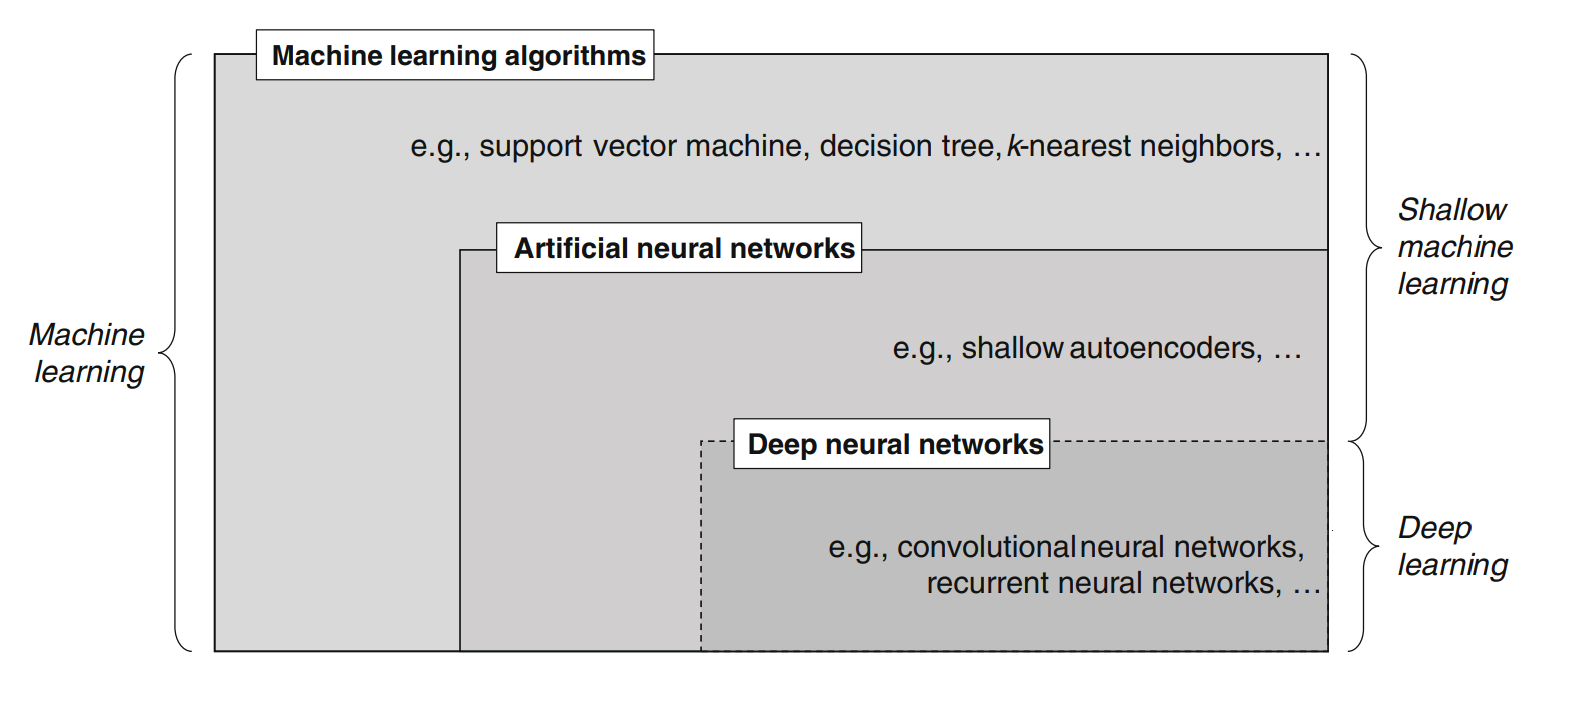
\includegraphics[width=15cm]{assets/images/ML_concepts}
\par\end{centering}
\caption{Landscape of Machine Learning concepts and methods \cite{janiesch2021machine}. \label{fig:ML_concepts}}
\end{figure}

\begin{longtable}{| p{0.2\textwidth} | p{0.8\textwidth} |}
    \hline
    \textbf{Type} & \textbf{Description} \\
    \hline
    Supervised learning &  A training dataset that includes instances for the input and labeled answers or target values for the output is required for supervised learning. This dataset must also include instances for the input. Taking into consideration the target variable, also known as the y variable, one example may be making a prediction regarding the amount of active users who will be subscribing to a marketplace platform in the next month. It is usual practice to refer to these qualities as input features or x variables. This prediction is based on a number of different input characteristics, such as the quantity of items that have been sold or positive customer reviews. The final step involves making use of the sets of input and output data that are contained within the training set in order to fine-tune the adjustable parameters of the machine learning model. After the training procedure for the model has been successfully completed, it will be able to make accurate predictions for the target variable y when it is given data points for the input characteristics x that it has not previously encountered. A more nuanced distinction can be made with regard to the category of supervised learning between regression problems, in which the objective is to forecast a numerical value (for example, the number of users), and classification problems, in which the anticipated outcome is a categorical class affiliation, such as "lookers" or "buyers." \\
    \hline
    Unsupervised learning & The process of unsupervised learning takes place when the learning system is given the goal of recognizing patterns without the existence of any pre-existing labels or requirements within the system. Within the scope of this discussion, the training data is comprised entirely of variables x, with the objective of elucidating structural information of interest. One example of this is the process of clustering, which involves discovering groups of items that share similar qualities. Another example is the process of dimensionality reduction, which involves producing data representations that are projected from a high-dimensional space into a lower-dimensional space. The use of clustering strategies is a noteworthy example of unsupervised learning in the context of electronic marketplaces. This strategy is utilized to categorize clients or markets into segments, which enables communication that is more targeted and specialized, as well as suited to the characteristics of each segment being targeted. \\
    \hline
    Reinforcement learning & In a reinforcement learning system, rather than providing input and output pairs, we outline the current state of the system, establish a goal, present a list of actions that are permitted along with the environmental constraints that they are subject to, and then allow the machine learning model to go through the process of achieving the goal on its own. In order to optimize a reward, this is accomplished through the use of the trial-and-error principle. There has been a significant amount of success obtained by reinforcement learning models in confined contexts such as games. Their usefulness, on the other hand, extends to multi-agent systems, such as electronic marketplaces with several agents. \\
    \hline
  \caption{Overview of types of machine learning. Taken from \cite{janiesch2021machine}}
  \label{tab:typesofML}
\end{longtable}

\subsection{\acrshort{ml} Applications}

In discerning which machine learning method(s) to employ, the initial step involves precisely formulating one's research question. Hernán and colleagues' framework introduces three primary data science research tasks: description, prediction, and causal inference.\cite{Hernan}. Machine learning is applicable to each of these three tasks; however, depending on the particular research question, conventional statistical methods might be adequate and more suitable.
\begin{itemize}
\item Description - Tasks related to description entail utilizing data to furnish a quantitative summary of specific variables. In description tasks, unsupervised machine learning methods prove especially beneficial as they strive to uncover relationships within a data structure without relying on a measured outcome. The objective of unsupervised learning is to discern underlying dimensions, components, clusters, or trajectories within a given data structure.

\item Prediction - The second prominent data science task is prediction, encompassing a variety of specific objectives. Conventional statistical methods, such as logistic regression, can be employed to test this hypothesis. They facilitate the acquisition of interpretable estimates regarding the nature and statistical significance of associations between predictors and the outcome, for instance, odds ratio. In scenarios where the objective is the optimization of prediction within large or complex data structures, machine learning might be favored over traditional statistical methods. This preference arises from the fact that machine learning methods have fewer and less restrictive statistical assumptions when compared to traditional parametric methods. A correlated objective in prediction is the identification of variables that significantly contribute to the accuracy of predictions.

Supervised learning emerges as the linchpin for articulating prediction tasks, driven by the ambition to adeptly forecast or classify specific outcomes of interest, such as discerning the presence or absence of a mental disorder. This strategic approach finds application in the expansive realm of data structures, weaving together a rich tapestry that spans demographic, clinical, and social predictors.

\item Causal Inference - Causal inference encompasses the nuanced process of estimating effects through a meticulous comparison of outcomes among individuals exposed to a particular factor and counterfactual outcomes that hypothesize what would have transpired had they not been exposed. This methodological approach is rooted in the discernment of causality, striving to unravel the true impact of an exposure by scrutinizing the divergence between observed outcomes and those counterfactual scenarios that serve as a baseline for comparison. Causal inference finds practical application in analyzing observational data, which lacks the randomization inherent in experimental designs, by adopting an approach that mirrors a hypothetical randomized trial. Although causal inference methods have been a longstanding presence in research for decades, the incorporation of supervised learning techniques represents a more recent and innovative development \cite{JIANG2020675}.
\end{itemize}



\subsection{\acrshort{dl} Applications}

\todo[inline]{Shorten each paragraph, remove too specific use cases}

\begin{enumerate}
    \item Natural language processing - \acrshort{dl} is used in natural language for voice translation, machine translation, and computer semantic comprehension, among other fields. In \cite{DONG2021100379}, Shi Dong concluded that \acrshort{dl} excels in image and natural language processing. Shi Dong cited 2015 Google Word Lens technology for real-time phone and video translation. This powerful technology may quickly recognize and translate words into the target language. The phone may also translate without an internet connection. Beyond visual translation, current technology can translate over 20 languages. Google added an automatic email reply capability to Gmail, using a DeepL model to evaluate email text.
    \item Speech recognition - Researchers worked hard to realize Human-Computer Interaction. By building the first experimental system in 1952, Davis and his Bell Institute team made history. This innovative approach identified 10 English digital pronunciations. Several decades have been spent researching speech recognition technologies, especially voice recognition. Voice recognition became a dominant force in some fields, named one of the top ten computer development events by the US press. Speech recognition technology has advanced significantly in the previous two decades. With the advancement of \acrshort{dl} models, several voice recognition devices and applications have moved from lab to market. Baidu \cite{Baidu} introduced Deep Speech in 2014, using \acrshort{dl} technology to achieve 8\% accuracy in noisy conditions. By February 2016, Baidu's Deep Speech 2 has lowered phrase recognition error rate to 3.7\%.
    \item Medical applications - \acrshort{dl}'s predicting and automated feature recognition make it a popular illness diagnostic approach. \acrshort{dl} uses in medicine, regardless of frequency or species, are constantly improving. Google began developing a groundbreaking technology to detect early-stage eye disorders in 2016. They sought early prevention of diabetic retinopathy and age-related macular degeneration with Moorfields Eye Hospital. A month later, Google developed a radiation approach for head and neck cancer using \acrshort{dl} methods. This novel method controlled radiation time and reduced injury risk. \acrshort{dl} technology is set to make significant contributions to precision medical treatment as it develops.

    \item Computer vision - Computer vision, a pivotal application within artificial intelligence, represents an interdisciplinary field dedicated to enabling computers to attain a sophisticated understanding from digital images or videos. This involves utilizing computers and cameras to substitute for the human eye in tasks such as target object recognition, tracking, measurement, and resolution of various visual challenges. Furthermore, it extends its purview to graphic processing, empowering computers to surpass the capabilities of the human eye in image processing.

    Below are listed the directions of computer vision.

    \begin{itemize}
        \item Image segmentation - Image segmentation doesn't need visual ideas or object recognition, unlike image categorization or object recognition. An object classifier only defines labeled items. In addition, an optimum picture segmentation algorithm segments new or unrecognized items. In human-computer interaction, each video frame is segmented to help users interact with people and objects. In an airport, the security crew focuses on unsecured objects that may contain dangerous compounds. This requires investigating all left-behind items.
        
        \item Face recognition - 
       Face recognition uses human face traits for biometric identification. The camera records video or picture data of the face, which is then used for automated image and face detection. The newest \acrshort{dl} algorithm, like FaceNet, achieves 99.63\% face recognition accuracy, exceeding eye recognition. \acrshort{dl} excels at capturing key features that manual expressions lack. Strong face attribute and identification selectivity and robustness for local blocks result from its moderate sparsity. \acrshort{dl} features are used for face recognition, with display limitations or post-processing incorporated. Integration of \acrshort{dl} is a key factor in its widespread use in face recognition. \acrshort{cnn} technology is crucial for facial recognition in \acrshort{dl}.
        
        \item Object detection - 
        Object detection identifies categories of objects in photos or videos, such as human faces and eyes. Object detection is essential to image understanding and computer vision, tackling complex problems including scene comprehension, picture captioning, event detection, and activity recognition. Its uses include consumer electronics, robot vision, security, autonomous driving, human-computer interaction, and automated surveillance. Due of image size, traditional algorithms have trouble learning patterns.
    
    \end{itemize}

    \item \acrshort{dl} on graphs - Recently, academics have begun developing new methods for discovering patterns from graph-structured data. \acrshort{dl} on graphs has been effective in tackling many challenges. 
    In 2017, Ktena et al. \cite{KTENA} used graph \acrshort{cnn} to predict graph similarity, detecting brain diseases. It is typical to treat complicated illnesses with numerous medications targeting intricate diseased proteins. However, changing one medicine may not be noticeable in clinical settings, especially with multiple drugs.

    \item \acrfull{its} - \acrshort{its} underpin smart cities and provide crucial infrastructure for governments across ages. Vehicle management, a major part of transportation networks, is becoming harder and requires robots. US people took 181,541 public transportation vehicles for 9.9 billion trips and 55.8+ billion kilometers in 2019. This high utilization emphasizes smart transportation's importance for large cities worldwide. Transportation data comes in several forms, including text, audio, photos, and videos \cite{DONG2021100379}.
    
\end{enumerate}

\subsection{Data input}
In addition to conventional numerical data, there is considerable volume of diverse data, particularly unstructured and non-cross-sectional data, including time series, images, and text. This data can be utilized for the construction of analytical models, aiming to enhance decision support or facilitate business automation purposes. Nevertheless, manually extracting patterns and relationships would surpass the cognitive capacity of human operators, underscoring the indispensability of algorithmic support, especially when dealing with large and high-dimensional datasets.

The latest advancements in \acrshort{dl} enable the processing of diverse types of data in combination, commonly known as cross-modal learning. This capability is valuable in applications where content is presented in multiple forms of representation, as seen in e-commerce websites where product information is typically conveyed through images, concise descriptions, and additional text metadata. Once these cross-modal representations are acquired, they can be employed, for instance, to enhance retrieval and recommendation tasks or to identify misinformation and fraud \cite{janiesch2021machine}.

\subsection{Feature extraction}

The extraction of features that may be used in the construction of models is an essential step in the process of automatically recognizing patterns and correlations within large amounts of data resources. In a general sense, a feature is a description of a characteristic that is derived from the initial data input with the intention of delivering an acceptable representation. As a result, the purpose of feature extraction is to maintain information that is discriminative and to discern between variables of variation that are pertinent to the overall learning goal.

The achievement of success in shallow machine learning is closely connected to the utilization of well specified features, and the performance of this technique is contingent upon the efficiency of the extraction process. The process of manually crafting features is a difficult task that often requires a significant amount of domain expertise inside a specialized engineering process that is suited to a particular application. It is considered to be laborious, time-consuming, and lacking in flexibility due to the fact that it requires a significant amount of effort.

\acrfull{dnn} address this constraint associated with manually crafted feature engineering. Their sophisticated structure empowers them with the ability to autonomously learn features, extracting discriminative representations with minimal human intervention. Hence, \acrshort{dl} is more adept at handling extensive, noisy, and unstructured datasets. The process of acquiring features typically advances in a hierarchical fashion, where more complex, high-level abstract features are constructed from simpler ones. 
However, based on the nature of the data and the selection of \acrshort{dl} architecture, various methods of feature learning are employed in tandem with the model-building phase \cite{janiesch2021machine}.

\subsection{Model building} 
In the process of automated model construction, a learning algorithm utilizes the input to discern patterns and relationships that are pertinent to the specific learning task. In contrast, \acrshort{dl} has the ability to directly work with high-dimensional raw input data for the purpose of model construction, leveraging its automated feature learning capability. Hence, architectures in \acrshort{dl} are frequently structured as end-to-end systems that integrate both aspects into a single pipeline.  Differences in architectural variants primarily stem from the kinds of layers, neural units, and connections they employ. Table \ref{tab:typesofDL} provides an overview of the three categories of \acrshort{cnn} \acrfull{rnn} and \acrshort{dnn} \cite{janiesch2021machine}.

\begin{table}[H]
  \centering
  \begin{tabular}{|p{3cm}|p{11cm}|}
    \hline
    \textbf{Architecture} & \textbf{Description} \\
    \hline
    \acrlong{cnn} & \acrshort{cnn} are predominantly employed in tasks associated with computer vision and speech recognition. They can tackle tasks that involve datasets with spatial relationships, where the interchangeability of columns and rows is not applicable. Their network structure consists of multiple stages, facilitating hierarchical feature learning in accordance with the specific modeling task at hand. As an illustration, in the context of object recognition in images, the initial layers of the network are tasked with extracting fundamental features, such as edges and corners. These basic features are progressively combined in the final layers to form more intricate representations resembling the actual objects of interest, such as animals, houses, or cars. \\
    \hline
    \acrlong{rnn} & \acrshort{rnn} are explicitly crafted for data structures that follow a sequence, such as time-series data, event sequences, and natural language. Their structure incorporates internal feedback loops, allowing for the learning of sequential patterns and the modeling of time dependencies by establishing a memory. Basic \acrshort{rnn} architectures pose challenges as they encounter the issue of vanishing gradients, leading to minimal or no impact from early memories. More advanced architectures, like long short-term memory (LSTM) networks equipped with sophisticated attention mechanisms, address this issue. \\
    \hline
    \acrlong{dnn} & \acrshort{dnn} are distinguished by the inclusion of a large number of hidden layers that are grouped in complex network designs. Their ability to handle raw input data and independently discover the representations that are necessary for the learning task is significantly improved as a result of their frequent utilization of complex processes, like as convolutions, or the incorporation of numerous activations inside a single neuron. \acrshort{dl} is the term that is usually used to describe this kind of capacity.\\
    \hline
  \end{tabular}
  \caption{Overview of \acrshort{dl} architectures. Taken from \cite{janiesch2021machine}}
  \label{tab:typesofDL}
\end{table}

\subsection{Model assessment}
Evaluating the quality of a model requires considering various aspects, including its performance, computational requirements, and interpretability. Metrics based on performance assess how effectively a model fulfills the objective set by the learning task. In the realm of supervised learning, there exist established guidelines for this particular endeavor. In this context, it is a standard practice to employ k-fold cross-validation to mitigate the risk of overfitting and assess the model's performance on out-of-sample data that was not part of the training set.

\begin{itemize}
\item
Regression - The evaluation of regression models involves assessing estimation errors, such as the root mean square error (RMSE) or the mean absolute percentage error (MAPE).

\item
Classification - The evaluation of classification models involves computing various ratios of correctly and incorrectly predicted instances, including accuracy, recall, precision, and the F1 score.

\end{itemize}

In choosing an appropriate prediction model for a given task, it is rational to compare different models with varying complexities. This involves considering competing model classes as well as alternative variants within the same model class. As previously mentioned, the complexity of a model can be described by several attributes, including the type of learning mechanisms (e.g., shallow machine learning vs. \acrshort{dl}), the quantity and type of manually created or autonomously extracted features, and the count of trainable parameters (e.g., network weights in artificial neural networks). Less complex models typically lack the flexibility to capture pertinent (non-linear) regularities and patterns associated with the learning task. On the flip side, excessively intricate models come with an increased likelihood of overfitting. Moreover, comprehending their reasoning is more challenging (as discussed in the next section), and they are likely to entail higher computational costs. The costs associated with computation are articulated through memory demands and the time taken for inference when executing a model on fresh data. These considerations are particularly crucial when assessing \acrshort{dnn}, given that processing and storing millions model parameters impose distinctive requirements on hardware resources. Hence, in business environments with limited resources, especially those heavily reliant on mobile devices, it is imperative to select a model that achieves a harmonious balance between underfitting and overfitting. 
They should also assess a model's complexity in terms of additional trade-off relationships, such as the balance between accuracy, memory usage, and speed.
\newline(\cite{janiesch2021machine})

\subsection{Balance in the model}

When constructing intelligent systems with shallow \acrshort{ml} and \acrshort{dl} models, the possibilities for algorithms or architectures, hyperparameters, and training data are virtually limitless(\cite{HEINRICH2021113494}). Simultaneously, there is a dearth of established guidelines regarding the construction of a model tailored for a specific problem. This lack extends to ensuring not only performance and cost-efficiency but also robustness and privacy. Furthermore, as described earlier, business environments with constrained resources frequently involve numerous trade-off relationships to contemplate, including the balance between prediction quality and computational costs. Hence, the process of constructing analytical models stands out as the most pivotal task, as it ultimately shapes the business success of an intelligent system. Comparisons between different implementations can be accurate only when altering one element of the triangle at a time and reporting identical metrics.
\newline(\cite{janiesch2021machine})


\section{Differential Privacy}

\acrfull{dp} conceals the presence or absence of any individual or small group of individuals within a dataset. This is accomplished by ensuring that, for each individual, any conclusion reached from the analysis would have been essentially as likely to have been reached regardless of whether the given individual joined the dataset or refrained from joining the dataset. In the following paragraphs will explain what \acrshort{dp} is, when it is appropriate to use it, how to implement it, and how to achieve it using frameworks. 

\subsection{Definition and characteristics of \acrshort{dp}}

\acrshort{dp} is a precise mathematical notion that provides a clear definition for protecting privacy. The story explores the interplay between a data analyst and a curator who has a dataset. The stipulation is a specific constraint on the probability of interactions across datasets that differ in the data of a single individual. This limitation hinders the exploration of new information on an individual's data, but it permits the gathering of statistical insights about all individuals in the dataset. Statistical learning reveals insights into cohorts of individuals, perhaps exposing information that members of the group may like to keep confidential. To do this, it is necessary to include a meticulously regulated level of unpredictability into the calculation. Therefore, the result of a differentially private analysis depends not only on the data itself but also on the added randomness. Essentially, after the dataset is completed, every possible outcome is linked to a probability that represents the chance of that outcome being seen. From the standpoint of individuals whose future is influenced by the algorithm's results, it may be stated that although it may be difficult to determine the likelihood of a subjectively negative outcome, the choice to participate or abstain from the data set will not substantially alter the risk. The term "significantly" is determined by the parameter $\varepsilon$, with a smaller value of $\varepsilon$ indicating less variation and so greater privacy. The change, whether it is an increase or a decrease, is multiplied by a factor of at most $e^\varepsilon$. When the value of $\varepsilon$ is significantly smaller than 1, the result is about 1 + $\varepsilon$. When $\varepsilon$ equals 1, the value is around 2.71. However, when $\varepsilon$ is more than 1, the value increases rapidly. For instance, when $\varepsilon$ is equal to 3, the value is about 20, and when $\varepsilon$ is equal to 5, it is approximately 148.4. When the value of $\varepsilon$ is equal to 15, it exceeds 3,269,017. When the value of the bound e is close to one (i.e., e is close to 0), any information obtained about a participant is about as likely to be obtained about a non-participant \cite{DWORK2019}.

The following four characteristics of \acrshort{dp} create an atmosphere that is particularly advantageous for data-driven and data-rich environments.

\begin{enumerate}
    \item An objective measurement of the loss of privacy that occurs as a result of \acrshort{dp} solutions may be made using. This allows for a comparative analysis of the risks to privacy posed by different systems. Although \acrshort{dp} may not always provide a clear distinction between high-quality and low-quality implementations, it does provide a chance to transform at least this aspect of an organization's privacy policies into a quality that can be evaluated by those who are not affiliated with the organization. Comparative analysis between different institutions is made possible by this quantification.
    \item Because of the requirement to choose $\varepsilon$, there is a chance to contemplate one's core beliefs. With the option to tweak $\varepsilon$, organizations are compelled to choose a privacy-utility mix and document it. This provides a database controller with the opportunity to modify her choice for privacy and utility. The controller might be the entity that owns or physically manages the database, or it could be a regulator that possesses logical control through a regulatory structure. Both of these possibilities are possible. In the process of algorithmic decision making, $\varepsilon$ generates a symbolic representation of social values as a placeholder.
    \item According to the mathematical definition of \acrshort{dp}, being differentially private is independent of what a privacy opponent may or might not know, as well as to which additional sources of information such an adversary might or might not have access, at any given moment, even in the future. This is the case regardless of whether the adversary is aware of the information or not. \acrshort{dp}, in other words, is not dependent on any one adversary and is future-proof.
    \item The mathematics of \acrshort{dp} makes it possible to monitor and manage the cumulative loss of privacy that occurs across many data uses \cite{DWORK2019}.
\end{enumerate}

\subsection{The Opposition of \acrshort{dp} in Action}

In addition to gaining a grasp of what \acrshort{dp} does give, it is essential to have an understanding of what it does not supply, even with a very small $\varepsilon$. \acrshort{dp} is not a single-solution solution. When it comes to studying outliers, \acrshort{dp} is not the appropriate instrument to utilize since it conceals the presence or absence of outliers. For the purpose of studying tiny datasets, this tool is not appropriate. It is possible for \acrshort{dp} to conceal significant disparities in tiny populations or subpopulations of interest, depending on the choice of epsilon. However, despite the fact that this may be seen as a restriction, it is actually a feature. It is important to keep in mind that \acrshort{dp} assures that any result that is made from the analysis would have been essentially as likely to have been reached with or without the data of any individual than it would have been otherwise. When compared to the situation with small datasets, we anticipate that statistical estimators that are run on large datasets will be more resistant to the addition or deletion of a data point. This is because large datasets include more information. When compared to situations in which the dataset is big, the likelihood of a substantial change in the value of the statistical estimator being brought about by the addition or removal of single individual from a small dataset is considerably higher. Despite the fact that it is less accurate, \acrshort{dp} is, in fact, functioning as it was designed to do, which is to conceal the presence or absence of an individual over the results of the study. Legal limits on data access, usage, and sharing can occasionally promote the correct mix between discovery and privacy in situations where tiny datasets need to be evaluated. This is the case if the intended application supports the confidentiality risks that are involved. Consider the possibility of a federal database that contains personally identifiable health information that has been gathered without the individual's agreement for the sake of public health, such as detecting persons who are infectious. Unlike informational privacy, this non-consensual collecting is not addressed by \acrshort{dp}, which is a violation of informational privacy. The additional information that is obtained from the analysis of the data that protects individuals' privacy may be used to modify the information that is provided to persons who are making significant decisions regarding their health care (for example, a decision regarding reproduction). This is another possible cause for worry. \acrshort{dp} does not in any way restrict the manner in which the information obtained about the population as a whole is utilized to impact the treatment of particular people, regardless of whether or not the data collected from those individuals were included in the database \cite{DWORK2019}.

\subsection{Exactly What Does Epsilon Mean?}

\subsubsection{An Uncertainty Regarding the Optimality}

There is a lack of clarity on the appropriate level of privacy loss in a particular setting, which works to weaken the pressure that is being put on for adequate \acrshort{dp} implementations. To begin, it is feasible that a procedure that may extract the highest potential utility for any given value of may simply not be known. This is true for a particular analytical activity in general as well as for a very specific type of data. Through the use of technical research, this issue can be resolved over time. The second issue is that we do not have a formula that can determine, given a particular privacy-utility tradeoff, what the most prudent choice of epsilon would be. As was seen in the flossing example, not all big epsilon are the same. This is especially relevant in light of the fact that.
If we do not know how small an epsilon is possible, which means how much privacy can be offered, consistent with a given analytical utility (the optimal privacy-utility mix), or if we do not know a fair privacy price to pay for what we learn, then the measurement has less meaning. This is because we are able to cap the amount of privacy loss that a particular algorithm can cause \cite{DWORK2019}.

\subsubsection{Understanding the Meanings of Epsilons of a Smaller Size}

Although all tiny epsilons are similar, it is important to keep in mind that the value of $e^\varepsilon$ is approximately equal to the sum of $\varepsilon$ and one, provided that $\varepsilon$ is less than one. This is based on an analogy to the first phrase of Anna Karenina, which states, "All happy families are alike, but an unhappy family is unhappy after its own fashion." This makes it difficult to reason about the huge $\varepsilon$, which states that each large $\varepsilon$ is enormous after its own fashion. Imagine that there are two different kinds of entities that live in this world: ghosts and humans. This means that both kinds of creatures behave in the same manner, interact with other people in the same manner, blog, study, work, laugh, love, mourn, reproduce, become ill, recover, and age in the same manner. There is just one distinction between ghosts and people, and that is that ghosts do not have any recordings in statistical databases. The enemy of privacy seeks to ascertain if a certain individual, who is fifty years old and is referred to as the "target," is a ghost or a human being. The enemy is, in fact, allowed the whole fifty years to do this. It is not necessary for the adversary to remain passive. For instance, she can organize clinical trials and enroll patients of her choosing. She can also create humans to populate databases, effectively creating the worst-case scenario (for privacy) databases that were discussed earlier. Furthermore, she can expose the target to chemicals at the age of 25 and again at the age of 35. Her knowledge of the target encompasses every single piece of information that could ever be recorded into any database. If the target were human, she would be able to determine which databases the target would be in. This would mean that the only potential violation of privacy that would be left to worry about would be the human/ghost bit of the target. In this particular scenario, every assurance of a constraint of  $\varepsilon$ on privacy loss is similar; the particular method and the kind of data are immaterial \cite{DWORK2019}.

When $\varepsilon$ is small, the human/ghost bit remains hidden, regardless of how much or how little additional information the adversary has about the target and about the rest of the world. This is true whether we are discussing a single computation or the cumulative privacy loss associated with multiple computations performed on the same database or across multiple databases. In this particular scenario, a tiny $\varepsilon$ guarantees that the database does not disclose any information about the target (beyond what would be disclosed about the target based on the outcome of the calculation in the event that the target had chosen to opt out of the dataset). We have seen that this unification is unsuccessful when the value of $\varepsilon$ is high, as demonstrated by the flossing example. From a mathematical standpoint, this is due to the fact that dealing with a big $\varepsilon$ simply does not succeed in concealing the human/ghost bit. As a result, we are unable to draw any conclusions from the assumption that this bit is concealed, just as we did in the case of a small $\varepsilon$. When $\varepsilon$ is small, decent reasoning regarding the semantics of \acrshort{dp}, including making sure that we are legitimately comparing apples to apples, is sound. However, when $\varepsilon$ is big, this reasoning is no longer sound \cite{DWORK2019}.

\subsection{\acrshort{dp} Mechanisms}

This is the time when we will talk about several well-known techniques of \acrshort{dp}.

\begin{itemize}
    \item Randomized Response Mechanism - The randomized response is an example of a non-interactive technique, in which the data of each user is affected in an individual manner based on the outcome of coin flips. This technique affords the respondent the opportunity to maintain "plausible deniability" \cite{RandRespMechanism}.
    \item Laplace Mechanism - In the field of \acrshort{dp}, the Laplace mechanism is among the mechanisms that are utilized the most frequently. According to this approach, the random noise that conforms to the Laplace distribution with a mean of zero and a sensitivity of $GS(f)/\varepsilon$ is incorporated into the answer of every query in order to ensure that it is disturbed in an acceptable manner \cite{LaplaceMechanism}. When calculating noise with l1 sensitivity, the Laplace technique is often utilized in $\varepsilon$ \acrshort{dp}. This is mostly due to the fact that $\varepsilon$ is the sole parameter that is of relevance. In addition, the bounded Laplace mechanism is utilized by GRAM-DP in order to incorporate noise into the query answer.
    \item Gaussian Mechanism - Another technique that has garnered a lot of interest in recent times is the Gaussian mechanism, which is designed to create ($\varepsilon$, $\delta$)-\acrshort{dp}. The answer of the query is now being supplemented with a certain quantity of zero-mean Gaussian noise. The quantity of noise that was added to the result corresponds to the sensitivity of the l2 scale. Along with $\varepsilon$, another component that plays a significant role in this context is $\delta$, which is responsible for determining the likelihood of one's privacy being compromised. The demonstration of an extended Gaussian method for \acrshort{dp} was carried out by Liu et al. \cite{GaussianMechanism}.
    \item Exponential Mechanism - There are some queries that do not supply their output with numerical numbers. Therefore, McSherry and Talwar \cite{ExpMechanism} developed a mechanism that can be utilized to make non-numerical searches differentially private. This method may be employed. Since the Exponential mechanism assigns exponentially larger odds of being picked for the higher outcomes, the end result would be near to optimal answers after applying it for nonnumeric inquiries. This is because the probability of being selected for the higher outcomes is exponentially higher.
    
\end{itemize} 

\subsection{\acrshort{dp} Frameworks}

Next table \ref{tab:frameworksDP} describes different DP frameworks.

\begin{longtable}{| p{0.25\textwidth} | p{0.8\textwidth} |}
    \hline
    \textbf{Framework} & \textbf{Description} \\
    \hline
    Opacus & In addition to being developed on top of PyTorch, the DP library for \acrshort{ml} services that Facebook uses is called PyTorch Opacus \cite{opacus1}. OpenMined is an open-source community that is committed to researching privacy strategies for machine learning and artificial intelligence. It is being developed in conjunction with Facebook AI Research, the PyTorch team, and OpenMined. Because of its broad and specialized qualities, the service offered by Opacus is geared for both professional DP researchers and practitioners of machine learning practice. \\
    \hline
    OpenDP & OpenDP Smartnoise \cite{opendp1} can trace its origins back to the Privacy Tools Project initiated by Harvard University. Through the course of this project, they were able to acquire expertise in the construction and deployment of PSI \cite{opendp2}, which is a system that was built to exchange and analyze privacy-sensitive datasets while maintaining the privacy safeguards of DP. Ultimately, this project helped to their efforts toward Smartnoise. Other distributed processing (DP) technologies, such as PinQ \cite{opendp3}, ektelo \cite{opendp4}, PrivateSQL \cite{opendp5}, Fuzz \cite{opendp6}, and LightDP \cite{opendp7}, have also been merged into OpenDP Smartnoise. Even though the majority of the tools, such as PSI and PinQ, are research prototypes, OpenDP Smartnoise is now putting up efforts to further develop DP principles into solutions that are ready for production utilization. As a result of these characteristics, OpenDP Smartnoise has garnered a great amount of popularity within the developer community, as evidenced by the fact that its open-source software repository has more than two hundred stars. \\
    \hline
    Google DP & An open-source version of Google's DP library, which is used to power several of the company's major products, was recently published by Google \cite{googledp1}. This library, which is available in Java and Go, is a collection of years' worth of developer experience from Google. It provides practitioners and organizations with the opportunity to reap possible advantages from its implementation, and it requires a relatively minimal degree of skill in DP to get started. \\
   
    \hline
    Tensorflow Privacy & The work of Abadi et al. \cite{tf-dp1}, who constructed a comparable optimizer for TensorFlow and a privacy cost tracker, served as the initial inspiration for the development and distribution of TensorFlow Privacy \cite{tf-dp2} (TFP), which is a machine learning framework developed and distributed by Google. The emergence and adaptation of DP mechanisms to TensorFlow is what makes it possible for users to take advantage of \acrshort{dp} when training machine learning models. Additionally, TFP is adjustable, and developers have the ability to create their own machine learning models. With these models, developers are able to develop their own operators and integrate them in their applications. Because of its adaptability and DP services, TFP has evolved into an open DP tool that is utilized by a sizable developer community and to which they provide significant contributions. \\
    \hline
    Diffprivlib & The industrial giant IBM is responsible for the development of Diffprivlib \cite{Diffprivlib1}, which enables \acrshort{dl} in machine learning tasks such as classification, regression, clustering, dimensionality reduction, and data regularization. A tool that may be used for a variety of purposes, including performing experiments, investigations, and application development while maintaining \acrshort{dl} is what it is intended to be. During their interactions with Diffprivlib, practitioners of varying levels will have no trouble locating the information they want thanks to the comprehensive product handbook that can be found at https://diffprivlib.readthedocs.io/en/latest/. This manual was accessed on December 31, 2023. The open repository that Diffprivlib maintains \cite{Diffprivlib2} has garnered a significant amount of attention from developers as a consequence of this. \\
    \hline
    Chorus & Chorus \cite{chorus1, chorus2} uses a cooperative architecture to conduct DP statistical queries. It uses industrial-grade database management systems (DBMS) for data processing and queries that need to be altered or repeated. This design focuses on rewriting, analysis, and postprocessing. The post-processing component processes query output, whereas the rewriting component changes queries for clipping. The analysis component analyzes queries to find features such \acrshort{dl} noise. Chorus' clipping summing procedure illustrates this. The rewriting component can modify the initial query such that the database management system (DBMS) clips and sums, while the analysis and post-processing component completes the summation. Chorus differs from previous efforts because of its DBMS independence. Chorus does not require database change or a server-based database engine, unlike an integrated solution. When working with large datasets, Chorus can employ DMBS to ensure scalability. Chorus deployment may require additional measures to prevent hostile actors from getting sensitive data. Chorus' Uber implementation restricted privacy-sensitive data to a central query interface. The UI, privacy budget account, and DMBS were protected against tampering. \\
    \hline
  \caption{Description of DP Frameworks \cite{zhang2023evaluation}}
  \label{tab:frameworksDP}
\end{longtable}




% Evaluation
\clearpage\null
\chapter{Evaluation \label{cha:eva}}



% Related Work
\clearpage\null
\chapter{Related Work}


% Conclusion
\clearpage\null
\chapter{Conclusion}

\section{Summary}


\section{Future Work}


% Resume
\clearpage\null

\chapter*{Resumé}


% Bibliography
\clearpage\null
\printbibliography[heading=references,segment=\therefsegment, resetnumbers=true]

\end{refsegment}

% Appendix
\appendix

\clearpage\null
\setcounter{figure}{0}
\setcounter{listing}{0}

\chapter{First Appendix \label{cha:chapter1} }

\begin{refsegment}

% Appendix
% \chapter{State Of The Art}

\section{Machine Learning \& Deep Learning}
\subsection{Introduction}
\acrfull{ml} strives to independently identify significant connections and patterns from instances and observations. Advances in \acrshort{ml} have paved the way for the recent development of intelligent systems that exhibit cognitive capabilities resembling those of humans. These systems have become integral in both our professional and personal lives. They play a crucial role in shaping the interconnected dynamics of electronic markets by improving decision-making processes for increased productivity, engagement, and employee retention in businesses. Furthermore, trainable assistant systems have the ability to customize themselves according to individual user preferences, while trading agents are causing disruptions in traditional finance markets \cite{janiesch2021machine}.

The success of these systems in addressing intricate issues, commonly known as artificial intelligence (AI), depends on analytical models that produce predictions, rules, responses, recommendations, or comparable results. Historically, attempts to construct these analytical models required the explicit programming of established relationships, procedures, and decision logic into intelligent systems using manually designed rules, such as expert systems for medical diagnoses. Due to the convenience offered by contemporary programming frameworks, ready access to data, and the widespread availability of computational power, analytical models are now more frequently created through a widely recognized approach referred to as \acrshort{ml}. \acrshort{ml} alleviates the workload on humans by removing the necessity to explicitly articulate and formalize knowledge in a format that machines can comprehend. This, in turn, streamlines the development of intelligent systems, making it more efficient \cite{janiesch2021machine}.

Over the past few decades, the domain of \acrshort{ml} has witnessed substantial advancements in improving sophisticated learning algorithms and applying effective pre-processing techniques. A notable accomplishment in this progression is the development of artificial neural networks (ANNs) towards more complex architectures, ultimately resulting in enhanced learning capabilities known as \acrfull{dl} \cite{janiesch2021machine}.


\subsection{Difference between \acrshort{ml} \& \acrshort{dl}}
Three core categories of \acrshort{ml} exists: supervised learning, unsupervised learning, and reinforcement learning.
Table \ref{tab:typesofML} contains a description of each of the three categories. 
The \acrshort{ml} field provides numerous classes of algorithms tailored to specific learning tasks, with each class having multiple specifications and variations. 
These include regression models, instance-based algorithms, decision trees, Bayesian methods, and artificial neural networks (ANNs) \cite{janiesch2021machine}. 

The versatility of the artificial neural network family is noteworthy, as its adaptable structure renders it suitable for a broad spectrum of applications within all three categories of machine learning. 
Mimicking the information processing principle observed in biological systems, artificial neural networks (ANNs) are composed of interconnected processing units known as artificial neurons. 
Like synapses in the brain, the connections between neurons relay signals, and the intensity of these signals can be adjusted by weights that undergo continuous modification throughout the learning process. 
Signals are processed by successive neurons only when they exceed a particular threshold, as dictated by an activation function. 
Neurons are commonly arranged into networks featuring distinct layers: an input layer that receives data input (such as product images), an output layer responsible for generating the final result (for instance, product categorization), and zero or more hidden layers tasked with learning non-linear mappings between the input and output \cite{janiesch2021machine}.

\acrshort{dl} proves particularly effective in domains with large and high-dimensional data, surpassing shallow \acrshort{ml} algorithms for tasks involving text, image, video, speech, and audio data. However, for low-dimensional input data, especially with limited training data availability, shallow \acrshort{ml} can still yield superior and more interpretable results compared to those generated by \acrfull{dnn} \cite{janiesch2021machine}.

Basic artificial neural networks and various machine learning algorithms fall into the category of shallow machine learning as they lack such capabilities. Since there is no precise boundary between the two concepts in the literature, we represent it with a dashed line in the Fig \ref{fig:ML_concepts}. While certain shallow machine learning algorithms are inherently interpretable to humans and are considered "white boxes," the decision-making process of most advanced machine learning algorithms is inherently untraceable unless explicitly explained. Therefore, it inherently constitutes a "black box" \cite{janiesch2021machine}.

\begin{figure}[H]
\begin{centering}
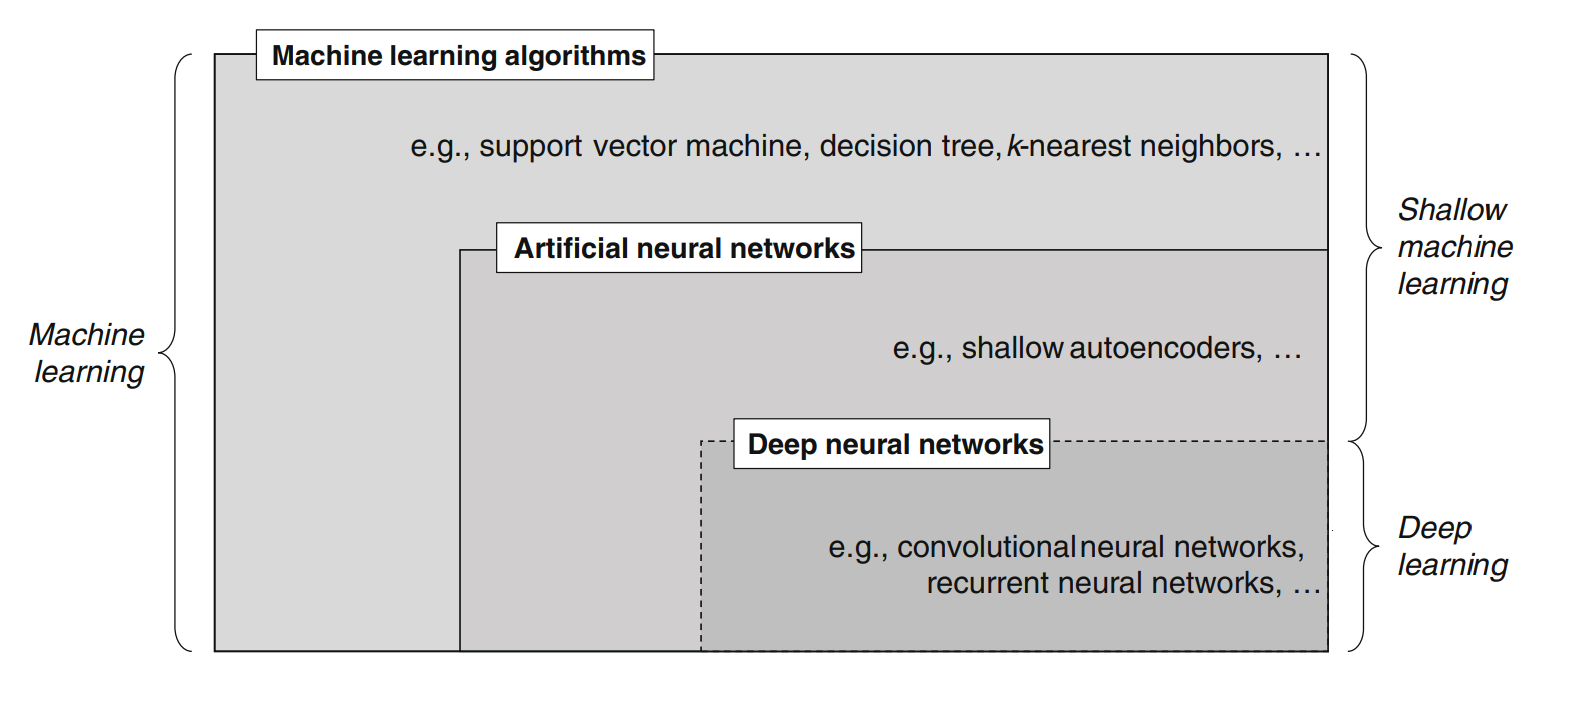
\includegraphics[width=15cm]{assets/images/ML_concepts}
\par\end{centering}
\caption{Landscape of Machine Learning concepts and methods \cite{janiesch2021machine}. \label{fig:ML_concepts}}
\end{figure}

\begin{longtable}{| p{0.2\textwidth} | p{0.8\textwidth} |}
    \hline
    \textbf{Type} & \textbf{Description} \\
    \hline
    Supervised learning &  A training dataset that includes instances for the input and labeled answers or target values for the output is required for supervised learning. This dataset must also include instances for the input. Taking into consideration the target variable, also known as the y variable, one example may be making a prediction regarding the amount of active users who will be subscribing to a marketplace platform in the next month. It is usual practice to refer to these qualities as input features or x variables. This prediction is based on a number of different input characteristics, such as the quantity of items that have been sold or positive customer reviews. The final step involves making use of the sets of input and output data that are contained within the training set in order to fine-tune the adjustable parameters of the machine learning model. After the training procedure for the model has been successfully completed, it will be able to make accurate predictions for the target variable y when it is given data points for the input characteristics x that it has not previously encountered. A more nuanced distinction can be made with regard to the category of supervised learning between regression problems, in which the objective is to forecast a numerical value (for example, the number of users), and classification problems, in which the anticipated outcome is a categorical class affiliation, such as "lookers" or "buyers." \\
    \hline
    Unsupervised learning & The process of unsupervised learning takes place when the learning system is given the goal of recognizing patterns without the existence of any pre-existing labels or requirements within the system. Within the scope of this discussion, the training data is comprised entirely of variables x, with the objective of elucidating structural information of interest. One example of this is the process of clustering, which involves discovering groups of items that share similar qualities. Another example is the process of dimensionality reduction, which involves producing data representations that are projected from a high-dimensional space into a lower-dimensional space. The use of clustering strategies is a noteworthy example of unsupervised learning in the context of electronic marketplaces. This strategy is utilized to categorize clients or markets into segments, which enables communication that is more targeted and specialized, as well as suited to the characteristics of each segment being targeted. \\
    \hline
    Reinforcement learning & In a reinforcement learning system, rather than providing input and output pairs, we outline the current state of the system, establish a goal, present a list of actions that are permitted along with the environmental constraints that they are subject to, and then allow the machine learning model to go through the process of achieving the goal on its own. In order to optimize a reward, this is accomplished through the use of the trial-and-error principle. There has been a significant amount of success obtained by reinforcement learning models in confined contexts such as games. Their usefulness, on the other hand, extends to multi-agent systems, such as electronic marketplaces with several agents. \\
    \hline
  \caption{Overview of types of machine learning. Taken from \cite{janiesch2021machine}}
  \label{tab:typesofML}
\end{longtable}

\subsection{\acrshort{ml} Applications}

In discerning which machine learning method(s) to employ, the initial step involves precisely formulating one's research question. Hernán and colleagues' framework introduces three primary data science research tasks: description, prediction, and causal inference.\cite{Hernan}. Machine learning is applicable to each of these three tasks; however, depending on the particular research question, conventional statistical methods might be adequate and more suitable.
\begin{itemize}
\item Description - Tasks related to description entail utilizing data to furnish a quantitative summary of specific variables. In description tasks, unsupervised machine learning methods prove especially beneficial as they strive to uncover relationships within a data structure without relying on a measured outcome. The objective of unsupervised learning is to discern underlying dimensions, components, clusters, or trajectories within a given data structure.

\item Prediction - The second prominent data science task is prediction, encompassing a variety of specific objectives. Conventional statistical methods, such as logistic regression, can be employed to test this hypothesis. They facilitate the acquisition of interpretable estimates regarding the nature and statistical significance of associations between predictors and the outcome, for instance, odds ratio. In scenarios where the objective is the optimization of prediction within large or complex data structures, machine learning might be favored over traditional statistical methods. This preference arises from the fact that machine learning methods have fewer and less restrictive statistical assumptions when compared to traditional parametric methods. A correlated objective in prediction is the identification of variables that significantly contribute to the accuracy of predictions.

Supervised learning emerges as the linchpin for articulating prediction tasks, driven by the ambition to adeptly forecast or classify specific outcomes of interest, such as discerning the presence or absence of a mental disorder. This strategic approach finds application in the expansive realm of data structures, weaving together a rich tapestry that spans demographic, clinical, and social predictors.

\item Causal Inference - Causal inference encompasses the nuanced process of estimating effects through a meticulous comparison of outcomes among individuals exposed to a particular factor and counterfactual outcomes that hypothesize what would have transpired had they not been exposed. This methodological approach is rooted in the discernment of causality, striving to unravel the true impact of an exposure by scrutinizing the divergence between observed outcomes and those counterfactual scenarios that serve as a baseline for comparison. Causal inference finds practical application in analyzing observational data, which lacks the randomization inherent in experimental designs, by adopting an approach that mirrors a hypothetical randomized trial. Although causal inference methods have been a longstanding presence in research for decades, the incorporation of supervised learning techniques represents a more recent and innovative development \cite{JIANG2020675}.
\end{itemize}



\subsection{\acrshort{dl} Applications}

\todo[inline]{Shorten each paragraph, remove too specific use cases}

\begin{enumerate}
    \item Natural language processing - \acrshort{dl} is used in natural language for voice translation, machine translation, and computer semantic comprehension, among other fields. In \cite{DONG2021100379}, Shi Dong concluded that \acrshort{dl} excels in image and natural language processing. Shi Dong cited 2015 Google Word Lens technology for real-time phone and video translation. This powerful technology may quickly recognize and translate words into the target language. The phone may also translate without an internet connection. Beyond visual translation, current technology can translate over 20 languages. Google added an automatic email reply capability to Gmail, using a DeepL model to evaluate email text.
    \item Speech recognition - Researchers worked hard to realize Human-Computer Interaction. By building the first experimental system in 1952, Davis and his Bell Institute team made history. This innovative approach identified 10 English digital pronunciations. Several decades have been spent researching speech recognition technologies, especially voice recognition. Voice recognition became a dominant force in some fields, named one of the top ten computer development events by the US press. Speech recognition technology has advanced significantly in the previous two decades. With the advancement of \acrshort{dl} models, several voice recognition devices and applications have moved from lab to market. Baidu \cite{Baidu} introduced Deep Speech in 2014, using \acrshort{dl} technology to achieve 8\% accuracy in noisy conditions. By February 2016, Baidu's Deep Speech 2 has lowered phrase recognition error rate to 3.7\%.
    \item Medical applications - \acrshort{dl}'s predicting and automated feature recognition make it a popular illness diagnostic approach. \acrshort{dl} uses in medicine, regardless of frequency or species, are constantly improving. Google began developing a groundbreaking technology to detect early-stage eye disorders in 2016. They sought early prevention of diabetic retinopathy and age-related macular degeneration with Moorfields Eye Hospital. A month later, Google developed a radiation approach for head and neck cancer using \acrshort{dl} methods. This novel method controlled radiation time and reduced injury risk. \acrshort{dl} technology is set to make significant contributions to precision medical treatment as it develops.

    \item Computer vision - Computer vision, a pivotal application within artificial intelligence, represents an interdisciplinary field dedicated to enabling computers to attain a sophisticated understanding from digital images or videos. This involves utilizing computers and cameras to substitute for the human eye in tasks such as target object recognition, tracking, measurement, and resolution of various visual challenges. Furthermore, it extends its purview to graphic processing, empowering computers to surpass the capabilities of the human eye in image processing.

    Below are listed the directions of computer vision.

    \begin{itemize}
        \item Image segmentation - Image segmentation doesn't need visual ideas or object recognition, unlike image categorization or object recognition. An object classifier only defines labeled items. In addition, an optimum picture segmentation algorithm segments new or unrecognized items. In human-computer interaction, each video frame is segmented to help users interact with people and objects. In an airport, the security crew focuses on unsecured objects that may contain dangerous compounds. This requires investigating all left-behind items.
        
        \item Face recognition - 
       Face recognition uses human face traits for biometric identification. The camera records video or picture data of the face, which is then used for automated image and face detection. The newest \acrshort{dl} algorithm, like FaceNet, achieves 99.63\% face recognition accuracy, exceeding eye recognition. \acrshort{dl} excels at capturing key features that manual expressions lack. Strong face attribute and identification selectivity and robustness for local blocks result from its moderate sparsity. \acrshort{dl} features are used for face recognition, with display limitations or post-processing incorporated. Integration of \acrshort{dl} is a key factor in its widespread use in face recognition. \acrshort{cnn} technology is crucial for facial recognition in \acrshort{dl}.
        
        \item Object detection - 
        Object detection identifies categories of objects in photos or videos, such as human faces and eyes. Object detection is essential to image understanding and computer vision, tackling complex problems including scene comprehension, picture captioning, event detection, and activity recognition. Its uses include consumer electronics, robot vision, security, autonomous driving, human-computer interaction, and automated surveillance. Due of image size, traditional algorithms have trouble learning patterns.
    
    \end{itemize}

    \item \acrshort{dl} on graphs - Recently, academics have begun developing new methods for discovering patterns from graph-structured data. \acrshort{dl} on graphs has been effective in tackling many challenges. 
    In 2017, Ktena et al. \cite{KTENA} used graph \acrshort{cnn} to predict graph similarity, detecting brain diseases. It is typical to treat complicated illnesses with numerous medications targeting intricate diseased proteins. However, changing one medicine may not be noticeable in clinical settings, especially with multiple drugs.

    \item \acrfull{its} - \acrshort{its} underpin smart cities and provide crucial infrastructure for governments across ages. Vehicle management, a major part of transportation networks, is becoming harder and requires robots. US people took 181,541 public transportation vehicles for 9.9 billion trips and 55.8+ billion kilometers in 2019. This high utilization emphasizes smart transportation's importance for large cities worldwide. Transportation data comes in several forms, including text, audio, photos, and videos \cite{DONG2021100379}.
    
\end{enumerate}

\subsection{Data input}
In addition to conventional numerical data, there is considerable volume of diverse data, particularly unstructured and non-cross-sectional data, including time series, images, and text. This data can be utilized for the construction of analytical models, aiming to enhance decision support or facilitate business automation purposes. Nevertheless, manually extracting patterns and relationships would surpass the cognitive capacity of human operators, underscoring the indispensability of algorithmic support, especially when dealing with large and high-dimensional datasets.

The latest advancements in \acrshort{dl} enable the processing of diverse types of data in combination, commonly known as cross-modal learning. This capability is valuable in applications where content is presented in multiple forms of representation, as seen in e-commerce websites where product information is typically conveyed through images, concise descriptions, and additional text metadata. Once these cross-modal representations are acquired, they can be employed, for instance, to enhance retrieval and recommendation tasks or to identify misinformation and fraud \cite{janiesch2021machine}.

\subsection{Feature extraction}

The extraction of features that may be used in the construction of models is an essential step in the process of automatically recognizing patterns and correlations within large amounts of data resources. In a general sense, a feature is a description of a characteristic that is derived from the initial data input with the intention of delivering an acceptable representation. As a result, the purpose of feature extraction is to maintain information that is discriminative and to discern between variables of variation that are pertinent to the overall learning goal.

The achievement of success in shallow machine learning is closely connected to the utilization of well specified features, and the performance of this technique is contingent upon the efficiency of the extraction process. The process of manually crafting features is a difficult task that often requires a significant amount of domain expertise inside a specialized engineering process that is suited to a particular application. It is considered to be laborious, time-consuming, and lacking in flexibility due to the fact that it requires a significant amount of effort.

\acrfull{dnn} address this constraint associated with manually crafted feature engineering. Their sophisticated structure empowers them with the ability to autonomously learn features, extracting discriminative representations with minimal human intervention. Hence, \acrshort{dl} is more adept at handling extensive, noisy, and unstructured datasets. The process of acquiring features typically advances in a hierarchical fashion, where more complex, high-level abstract features are constructed from simpler ones. 
However, based on the nature of the data and the selection of \acrshort{dl} architecture, various methods of feature learning are employed in tandem with the model-building phase \cite{janiesch2021machine}.

\subsection{Model building} 
In the process of automated model construction, a learning algorithm utilizes the input to discern patterns and relationships that are pertinent to the specific learning task. In contrast, \acrshort{dl} has the ability to directly work with high-dimensional raw input data for the purpose of model construction, leveraging its automated feature learning capability. Hence, architectures in \acrshort{dl} are frequently structured as end-to-end systems that integrate both aspects into a single pipeline.  Differences in architectural variants primarily stem from the kinds of layers, neural units, and connections they employ. Table \ref{tab:typesofDL} provides an overview of the three categories of \acrshort{cnn} \acrfull{rnn} and \acrshort{dnn} \cite{janiesch2021machine}.

\begin{table}[H]
  \centering
  \begin{tabular}{|p{3cm}|p{11cm}|}
    \hline
    \textbf{Architecture} & \textbf{Description} \\
    \hline
    \acrlong{cnn} & \acrshort{cnn} are predominantly employed in tasks associated with computer vision and speech recognition. They can tackle tasks that involve datasets with spatial relationships, where the interchangeability of columns and rows is not applicable. Their network structure consists of multiple stages, facilitating hierarchical feature learning in accordance with the specific modeling task at hand. As an illustration, in the context of object recognition in images, the initial layers of the network are tasked with extracting fundamental features, such as edges and corners. These basic features are progressively combined in the final layers to form more intricate representations resembling the actual objects of interest, such as animals, houses, or cars. \\
    \hline
    \acrlong{rnn} & \acrshort{rnn} are explicitly crafted for data structures that follow a sequence, such as time-series data, event sequences, and natural language. Their structure incorporates internal feedback loops, allowing for the learning of sequential patterns and the modeling of time dependencies by establishing a memory. Basic \acrshort{rnn} architectures pose challenges as they encounter the issue of vanishing gradients, leading to minimal or no impact from early memories. More advanced architectures, like long short-term memory (LSTM) networks equipped with sophisticated attention mechanisms, address this issue. \\
    \hline
    \acrlong{dnn} & \acrshort{dnn} are distinguished by the inclusion of a large number of hidden layers that are grouped in complex network designs. Their ability to handle raw input data and independently discover the representations that are necessary for the learning task is significantly improved as a result of their frequent utilization of complex processes, like as convolutions, or the incorporation of numerous activations inside a single neuron. \acrshort{dl} is the term that is usually used to describe this kind of capacity.\\
    \hline
  \end{tabular}
  \caption{Overview of \acrshort{dl} architectures. Taken from \cite{janiesch2021machine}}
  \label{tab:typesofDL}
\end{table}

\subsection{Model assessment}
Evaluating the quality of a model requires considering various aspects, including its performance, computational requirements, and interpretability. Metrics based on performance assess how effectively a model fulfills the objective set by the learning task. In the realm of supervised learning, there exist established guidelines for this particular endeavor. In this context, it is a standard practice to employ k-fold cross-validation to mitigate the risk of overfitting and assess the model's performance on out-of-sample data that was not part of the training set.

\begin{itemize}
\item
Regression - The evaluation of regression models involves assessing estimation errors, such as the root mean square error (RMSE) or the mean absolute percentage error (MAPE).

\item
Classification - The evaluation of classification models involves computing various ratios of correctly and incorrectly predicted instances, including accuracy, recall, precision, and the F1 score.

\end{itemize}

In choosing an appropriate prediction model for a given task, it is rational to compare different models with varying complexities. This involves considering competing model classes as well as alternative variants within the same model class. As previously mentioned, the complexity of a model can be described by several attributes, including the type of learning mechanisms (e.g., shallow machine learning vs. \acrshort{dl}), the quantity and type of manually created or autonomously extracted features, and the count of trainable parameters (e.g., network weights in artificial neural networks). Less complex models typically lack the flexibility to capture pertinent (non-linear) regularities and patterns associated with the learning task. On the flip side, excessively intricate models come with an increased likelihood of overfitting. Moreover, comprehending their reasoning is more challenging (as discussed in the next section), and they are likely to entail higher computational costs. The costs associated with computation are articulated through memory demands and the time taken for inference when executing a model on fresh data. These considerations are particularly crucial when assessing \acrshort{dnn}, given that processing and storing millions model parameters impose distinctive requirements on hardware resources. Hence, in business environments with limited resources, especially those heavily reliant on mobile devices, it is imperative to select a model that achieves a harmonious balance between underfitting and overfitting. 
They should also assess a model's complexity in terms of additional trade-off relationships, such as the balance between accuracy, memory usage, and speed.
\newline(\cite{janiesch2021machine})

\subsection{Balance in the model}

When constructing intelligent systems with shallow \acrshort{ml} and \acrshort{dl} models, the possibilities for algorithms or architectures, hyperparameters, and training data are virtually limitless(\cite{HEINRICH2021113494}). Simultaneously, there is a dearth of established guidelines regarding the construction of a model tailored for a specific problem. This lack extends to ensuring not only performance and cost-efficiency but also robustness and privacy. Furthermore, as described earlier, business environments with constrained resources frequently involve numerous trade-off relationships to contemplate, including the balance between prediction quality and computational costs. Hence, the process of constructing analytical models stands out as the most pivotal task, as it ultimately shapes the business success of an intelligent system. Comparisons between different implementations can be accurate only when altering one element of the triangle at a time and reporting identical metrics.
\newline(\cite{janiesch2021machine})


\section{Differential Privacy}

\acrfull{dp} conceals the presence or absence of any individual or small group of individuals within a dataset. This is accomplished by ensuring that, for each individual, any conclusion reached from the analysis would have been essentially as likely to have been reached regardless of whether the given individual joined the dataset or refrained from joining the dataset. In the following paragraphs will explain what \acrshort{dp} is, when it is appropriate to use it, how to implement it, and how to achieve it using frameworks. 

\subsection{Definition and characteristics of \acrshort{dp}}

\acrshort{dp} is a precise mathematical notion that provides a clear definition for protecting privacy. The story explores the interplay between a data analyst and a curator who has a dataset. The stipulation is a specific constraint on the probability of interactions across datasets that differ in the data of a single individual. This limitation hinders the exploration of new information on an individual's data, but it permits the gathering of statistical insights about all individuals in the dataset. Statistical learning reveals insights into cohorts of individuals, perhaps exposing information that members of the group may like to keep confidential. To do this, it is necessary to include a meticulously regulated level of unpredictability into the calculation. Therefore, the result of a differentially private analysis depends not only on the data itself but also on the added randomness. Essentially, after the dataset is completed, every possible outcome is linked to a probability that represents the chance of that outcome being seen. From the standpoint of individuals whose future is influenced by the algorithm's results, it may be stated that although it may be difficult to determine the likelihood of a subjectively negative outcome, the choice to participate or abstain from the data set will not substantially alter the risk. The term "significantly" is determined by the parameter $\varepsilon$, with a smaller value of $\varepsilon$ indicating less variation and so greater privacy. The change, whether it is an increase or a decrease, is multiplied by a factor of at most $e^\varepsilon$. When the value of $\varepsilon$ is significantly smaller than 1, the result is about 1 + $\varepsilon$. When $\varepsilon$ equals 1, the value is around 2.71. However, when $\varepsilon$ is more than 1, the value increases rapidly. For instance, when $\varepsilon$ is equal to 3, the value is about 20, and when $\varepsilon$ is equal to 5, it is approximately 148.4. When the value of $\varepsilon$ is equal to 15, it exceeds 3,269,017. When the value of the bound e is close to one (i.e., e is close to 0), any information obtained about a participant is about as likely to be obtained about a non-participant \cite{DWORK2019}.

The following four characteristics of \acrshort{dp} create an atmosphere that is particularly advantageous for data-driven and data-rich environments.

\begin{enumerate}
    \item An objective measurement of the loss of privacy that occurs as a result of \acrshort{dp} solutions may be made using. This allows for a comparative analysis of the risks to privacy posed by different systems. Although \acrshort{dp} may not always provide a clear distinction between high-quality and low-quality implementations, it does provide a chance to transform at least this aspect of an organization's privacy policies into a quality that can be evaluated by those who are not affiliated with the organization. Comparative analysis between different institutions is made possible by this quantification.
    \item Because of the requirement to choose $\varepsilon$, there is a chance to contemplate one's core beliefs. With the option to tweak $\varepsilon$, organizations are compelled to choose a privacy-utility mix and document it. This provides a database controller with the opportunity to modify her choice for privacy and utility. The controller might be the entity that owns or physically manages the database, or it could be a regulator that possesses logical control through a regulatory structure. Both of these possibilities are possible. In the process of algorithmic decision making, $\varepsilon$ generates a symbolic representation of social values as a placeholder.
    \item According to the mathematical definition of \acrshort{dp}, being differentially private is independent of what a privacy opponent may or might not know, as well as to which additional sources of information such an adversary might or might not have access, at any given moment, even in the future. This is the case regardless of whether the adversary is aware of the information or not. \acrshort{dp}, in other words, is not dependent on any one adversary and is future-proof.
    \item The mathematics of \acrshort{dp} makes it possible to monitor and manage the cumulative loss of privacy that occurs across many data uses \cite{DWORK2019}.
\end{enumerate}

\subsection{The Opposition of \acrshort{dp} in Action}

In addition to gaining a grasp of what \acrshort{dp} does give, it is essential to have an understanding of what it does not supply, even with a very small $\varepsilon$. \acrshort{dp} is not a single-solution solution. When it comes to studying outliers, \acrshort{dp} is not the appropriate instrument to utilize since it conceals the presence or absence of outliers. For the purpose of studying tiny datasets, this tool is not appropriate. It is possible for \acrshort{dp} to conceal significant disparities in tiny populations or subpopulations of interest, depending on the choice of epsilon. However, despite the fact that this may be seen as a restriction, it is actually a feature. It is important to keep in mind that \acrshort{dp} assures that any result that is made from the analysis would have been essentially as likely to have been reached with or without the data of any individual than it would have been otherwise. When compared to the situation with small datasets, we anticipate that statistical estimators that are run on large datasets will be more resistant to the addition or deletion of a data point. This is because large datasets include more information. When compared to situations in which the dataset is big, the likelihood of a substantial change in the value of the statistical estimator being brought about by the addition or removal of single individual from a small dataset is considerably higher. Despite the fact that it is less accurate, \acrshort{dp} is, in fact, functioning as it was designed to do, which is to conceal the presence or absence of an individual over the results of the study. Legal limits on data access, usage, and sharing can occasionally promote the correct mix between discovery and privacy in situations where tiny datasets need to be evaluated. This is the case if the intended application supports the confidentiality risks that are involved. Consider the possibility of a federal database that contains personally identifiable health information that has been gathered without the individual's agreement for the sake of public health, such as detecting persons who are infectious. Unlike informational privacy, this non-consensual collecting is not addressed by \acrshort{dp}, which is a violation of informational privacy. The additional information that is obtained from the analysis of the data that protects individuals' privacy may be used to modify the information that is provided to persons who are making significant decisions regarding their health care (for example, a decision regarding reproduction). This is another possible cause for worry. \acrshort{dp} does not in any way restrict the manner in which the information obtained about the population as a whole is utilized to impact the treatment of particular people, regardless of whether or not the data collected from those individuals were included in the database \cite{DWORK2019}.

\subsection{Exactly What Does Epsilon Mean?}

\subsubsection{An Uncertainty Regarding the Optimality}

There is a lack of clarity on the appropriate level of privacy loss in a particular setting, which works to weaken the pressure that is being put on for adequate \acrshort{dp} implementations. To begin, it is feasible that a procedure that may extract the highest potential utility for any given value of may simply not be known. This is true for a particular analytical activity in general as well as for a very specific type of data. Through the use of technical research, this issue can be resolved over time. The second issue is that we do not have a formula that can determine, given a particular privacy-utility tradeoff, what the most prudent choice of epsilon would be. As was seen in the flossing example, not all big epsilon are the same. This is especially relevant in light of the fact that.
If we do not know how small an epsilon is possible, which means how much privacy can be offered, consistent with a given analytical utility (the optimal privacy-utility mix), or if we do not know a fair privacy price to pay for what we learn, then the measurement has less meaning. This is because we are able to cap the amount of privacy loss that a particular algorithm can cause \cite{DWORK2019}.

\subsubsection{Understanding the Meanings of Epsilons of a Smaller Size}

Although all tiny epsilons are similar, it is important to keep in mind that the value of $e^\varepsilon$ is approximately equal to the sum of $\varepsilon$ and one, provided that $\varepsilon$ is less than one. This is based on an analogy to the first phrase of Anna Karenina, which states, "All happy families are alike, but an unhappy family is unhappy after its own fashion." This makes it difficult to reason about the huge $\varepsilon$, which states that each large $\varepsilon$ is enormous after its own fashion. Imagine that there are two different kinds of entities that live in this world: ghosts and humans. This means that both kinds of creatures behave in the same manner, interact with other people in the same manner, blog, study, work, laugh, love, mourn, reproduce, become ill, recover, and age in the same manner. There is just one distinction between ghosts and people, and that is that ghosts do not have any recordings in statistical databases. The enemy of privacy seeks to ascertain if a certain individual, who is fifty years old and is referred to as the "target," is a ghost or a human being. The enemy is, in fact, allowed the whole fifty years to do this. It is not necessary for the adversary to remain passive. For instance, she can organize clinical trials and enroll patients of her choosing. She can also create humans to populate databases, effectively creating the worst-case scenario (for privacy) databases that were discussed earlier. Furthermore, she can expose the target to chemicals at the age of 25 and again at the age of 35. Her knowledge of the target encompasses every single piece of information that could ever be recorded into any database. If the target were human, she would be able to determine which databases the target would be in. This would mean that the only potential violation of privacy that would be left to worry about would be the human/ghost bit of the target. In this particular scenario, every assurance of a constraint of  $\varepsilon$ on privacy loss is similar; the particular method and the kind of data are immaterial \cite{DWORK2019}.

When $\varepsilon$ is small, the human/ghost bit remains hidden, regardless of how much or how little additional information the adversary has about the target and about the rest of the world. This is true whether we are discussing a single computation or the cumulative privacy loss associated with multiple computations performed on the same database or across multiple databases. In this particular scenario, a tiny $\varepsilon$ guarantees that the database does not disclose any information about the target (beyond what would be disclosed about the target based on the outcome of the calculation in the event that the target had chosen to opt out of the dataset). We have seen that this unification is unsuccessful when the value of $\varepsilon$ is high, as demonstrated by the flossing example. From a mathematical standpoint, this is due to the fact that dealing with a big $\varepsilon$ simply does not succeed in concealing the human/ghost bit. As a result, we are unable to draw any conclusions from the assumption that this bit is concealed, just as we did in the case of a small $\varepsilon$. When $\varepsilon$ is small, decent reasoning regarding the semantics of \acrshort{dp}, including making sure that we are legitimately comparing apples to apples, is sound. However, when $\varepsilon$ is big, this reasoning is no longer sound \cite{DWORK2019}.

\subsection{\acrshort{dp} Mechanisms}

This is the time when we will talk about several well-known techniques of \acrshort{dp}.

\begin{itemize}
    \item Randomized Response Mechanism - The randomized response is an example of a non-interactive technique, in which the data of each user is affected in an individual manner based on the outcome of coin flips. This technique affords the respondent the opportunity to maintain "plausible deniability" \cite{RandRespMechanism}.
    \item Laplace Mechanism - In the field of \acrshort{dp}, the Laplace mechanism is among the mechanisms that are utilized the most frequently. According to this approach, the random noise that conforms to the Laplace distribution with a mean of zero and a sensitivity of $GS(f)/\varepsilon$ is incorporated into the answer of every query in order to ensure that it is disturbed in an acceptable manner \cite{LaplaceMechanism}. When calculating noise with l1 sensitivity, the Laplace technique is often utilized in $\varepsilon$ \acrshort{dp}. This is mostly due to the fact that $\varepsilon$ is the sole parameter that is of relevance. In addition, the bounded Laplace mechanism is utilized by GRAM-DP in order to incorporate noise into the query answer.
    \item Gaussian Mechanism - Another technique that has garnered a lot of interest in recent times is the Gaussian mechanism, which is designed to create ($\varepsilon$, $\delta$)-\acrshort{dp}. The answer of the query is now being supplemented with a certain quantity of zero-mean Gaussian noise. The quantity of noise that was added to the result corresponds to the sensitivity of the l2 scale. Along with $\varepsilon$, another component that plays a significant role in this context is $\delta$, which is responsible for determining the likelihood of one's privacy being compromised. The demonstration of an extended Gaussian method for \acrshort{dp} was carried out by Liu et al. \cite{GaussianMechanism}.
    \item Exponential Mechanism - There are some queries that do not supply their output with numerical numbers. Therefore, McSherry and Talwar \cite{ExpMechanism} developed a mechanism that can be utilized to make non-numerical searches differentially private. This method may be employed. Since the Exponential mechanism assigns exponentially larger odds of being picked for the higher outcomes, the end result would be near to optimal answers after applying it for nonnumeric inquiries. This is because the probability of being selected for the higher outcomes is exponentially higher.
    
\end{itemize} 

\subsection{\acrshort{dp} Frameworks}

Next table \ref{tab:frameworksDP} describes different DP frameworks.

\begin{longtable}{| p{0.25\textwidth} | p{0.8\textwidth} |}
    \hline
    \textbf{Framework} & \textbf{Description} \\
    \hline
    Opacus & In addition to being developed on top of PyTorch, the DP library for \acrshort{ml} services that Facebook uses is called PyTorch Opacus \cite{opacus1}. OpenMined is an open-source community that is committed to researching privacy strategies for machine learning and artificial intelligence. It is being developed in conjunction with Facebook AI Research, the PyTorch team, and OpenMined. Because of its broad and specialized qualities, the service offered by Opacus is geared for both professional DP researchers and practitioners of machine learning practice. \\
    \hline
    OpenDP & OpenDP Smartnoise \cite{opendp1} can trace its origins back to the Privacy Tools Project initiated by Harvard University. Through the course of this project, they were able to acquire expertise in the construction and deployment of PSI \cite{opendp2}, which is a system that was built to exchange and analyze privacy-sensitive datasets while maintaining the privacy safeguards of DP. Ultimately, this project helped to their efforts toward Smartnoise. Other distributed processing (DP) technologies, such as PinQ \cite{opendp3}, ektelo \cite{opendp4}, PrivateSQL \cite{opendp5}, Fuzz \cite{opendp6}, and LightDP \cite{opendp7}, have also been merged into OpenDP Smartnoise. Even though the majority of the tools, such as PSI and PinQ, are research prototypes, OpenDP Smartnoise is now putting up efforts to further develop DP principles into solutions that are ready for production utilization. As a result of these characteristics, OpenDP Smartnoise has garnered a great amount of popularity within the developer community, as evidenced by the fact that its open-source software repository has more than two hundred stars. \\
    \hline
    Google DP & An open-source version of Google's DP library, which is used to power several of the company's major products, was recently published by Google \cite{googledp1}. This library, which is available in Java and Go, is a collection of years' worth of developer experience from Google. It provides practitioners and organizations with the opportunity to reap possible advantages from its implementation, and it requires a relatively minimal degree of skill in DP to get started. \\
   
    \hline
    Tensorflow Privacy & The work of Abadi et al. \cite{tf-dp1}, who constructed a comparable optimizer for TensorFlow and a privacy cost tracker, served as the initial inspiration for the development and distribution of TensorFlow Privacy \cite{tf-dp2} (TFP), which is a machine learning framework developed and distributed by Google. The emergence and adaptation of DP mechanisms to TensorFlow is what makes it possible for users to take advantage of \acrshort{dp} when training machine learning models. Additionally, TFP is adjustable, and developers have the ability to create their own machine learning models. With these models, developers are able to develop their own operators and integrate them in their applications. Because of its adaptability and DP services, TFP has evolved into an open DP tool that is utilized by a sizable developer community and to which they provide significant contributions. \\
    \hline
    Diffprivlib & The industrial giant IBM is responsible for the development of Diffprivlib \cite{Diffprivlib1}, which enables \acrshort{dl} in machine learning tasks such as classification, regression, clustering, dimensionality reduction, and data regularization. A tool that may be used for a variety of purposes, including performing experiments, investigations, and application development while maintaining \acrshort{dl} is what it is intended to be. During their interactions with Diffprivlib, practitioners of varying levels will have no trouble locating the information they want thanks to the comprehensive product handbook that can be found at https://diffprivlib.readthedocs.io/en/latest/. This manual was accessed on December 31, 2023. The open repository that Diffprivlib maintains \cite{Diffprivlib2} has garnered a significant amount of attention from developers as a consequence of this. \\
    \hline
    Chorus & Chorus \cite{chorus1, chorus2} uses a cooperative architecture to conduct DP statistical queries. It uses industrial-grade database management systems (DBMS) for data processing and queries that need to be altered or repeated. This design focuses on rewriting, analysis, and postprocessing. The post-processing component processes query output, whereas the rewriting component changes queries for clipping. The analysis component analyzes queries to find features such \acrshort{dl} noise. Chorus' clipping summing procedure illustrates this. The rewriting component can modify the initial query such that the database management system (DBMS) clips and sums, while the analysis and post-processing component completes the summation. Chorus differs from previous efforts because of its DBMS independence. Chorus does not require database change or a server-based database engine, unlike an integrated solution. When working with large datasets, Chorus can employ DMBS to ensure scalability. Chorus deployment may require additional measures to prevent hostile actors from getting sensitive data. Chorus' Uber implementation restricted privacy-sensitive data to a central query interface. The UI, privacy budget account, and DMBS were protected against tampering. \\
    \hline
  \caption{Description of DP Frameworks \cite{zhang2023evaluation}}
  \label{tab:frameworksDP}
\end{longtable}




% Bibliography
\printbibliography[heading=referencessec,segment=\therefsegment,resetnumbers=true]

\end{refsegment}

\clearpage\null
\chapter{Contents of Included CD–ROM \label{cha:cdrom} }

CD–ROM included to the thesis contains following files:

\begin{itemize}
\item \texttt{/file1} --- First file
\item \texttt{/file2} --- Second file
\end{itemize}


\end{document}
